\section{Methodology} \label{sec3}

In the previous section some issues were identified with the dataset. The \textit{Algorithms and Techniques} subsection details the algorithms that were used to remedy these issues. In this section we show the results that were acquired during data preprocessing.

The other important contribution of this section is the feature engineering part. This provides details about how the features from the dataset were extracted.

\subsection{Preprocessing the Portfolio Dataset}

We do not use much data about the portfolio dataset. We do realize that some interesting features could have also been extracted from this data, however we decided to focus on other features of the data. In the full created feature vectors the offer that was received is one-hot-encoded to be able to feed it to the neural network. Also the duration of the offers is converted to hours to be able to use it with the transcript dataset where the timestamp is provided in hours instead of days.

\subsection{Preprocessing the Profile Dataset}

Due to the reasons detailed in the previous section we removed the people who have spent more than a total of 300\$ or did not spend anything. With this we have removed 6.8\% of the profile and and 7.3\% of the transcript data. These are not very large percentages, so there are plenty of data remaining after this selection.

After this, we have one-hot-encoded the gender into the following categories: "F", "M", "O" and "U". 

Before filling up the "None" type values in the dataset, the age and income fields are standardized using sklearn's StandardScaler algorithm. The features before and after standardization can be seen on Figure \ref{fig9}

\begin{figure}[h]
	\centering
	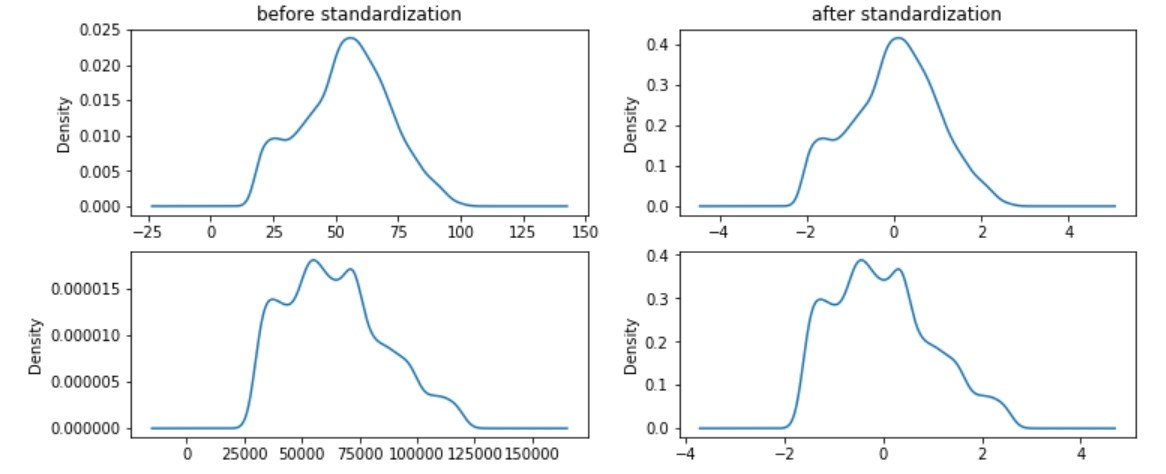
\includegraphics[width=0.8\textwidth]{fig/age_before_after.jpg}
	\vspace*{-0.1in}
	\caption{Age and income before and after standardization}
	\label{fig9}
	\vspace*{-0.2in}
	\bigskip
\end{figure}

After standardizing the age and income data, the missing values can be filled with the respective means. 

Next the membership length is calculated and since it was shown that it has a quite distorted distribution, it will be transformed using sklenarn's QuintileTransform algorithm. After that the resultant data is also standardized. The data before and after the transformation can be examined in Figure \ref{fig10}.

\begin{figure}[h]
	\centering
	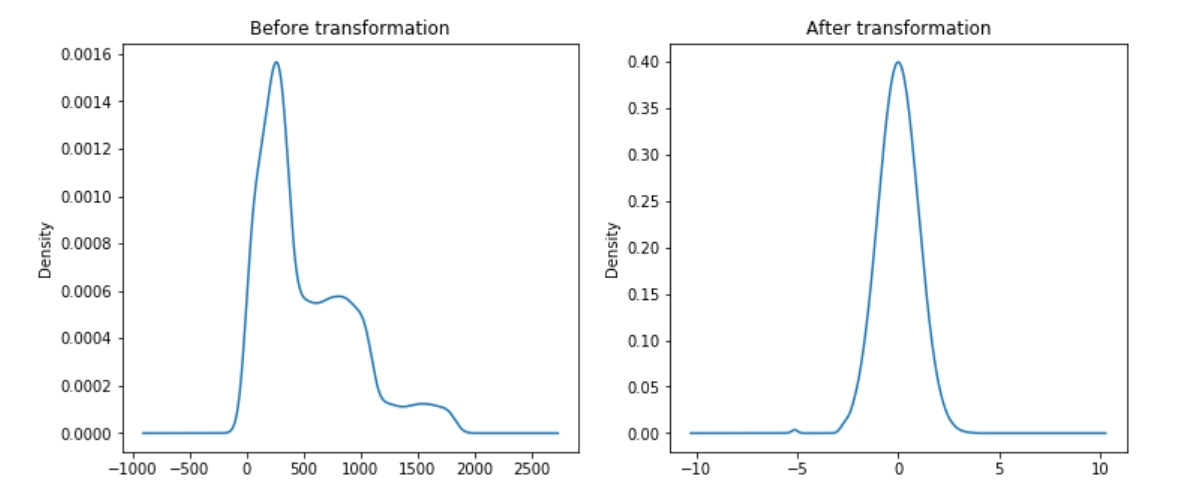
\includegraphics[width=0.8\textwidth]{fig/membership_before_after.jpg}
	\vspace*{-0.1in}
	\caption{Membership length before and after the transformation and standardization.}
	\label{fig10}
	\vspace*{-0.2in}
	\bigskip
\end{figure}

After the data was preprocessed and cleaned it is ready for handcrafted feature creation.

\section{Handcrafted Features}


